% $HeadURL$

%%%%%%%%%%%%%%%%%%%%%%%%%%%%%%%%%%%%%%%%%%%%%%%%%%%%%%%%%%%%%%%%%%%%%%
%%%%                   Compartment
%%%%%%%%%%%%%%%%%%%%%%%%%%%%%%%%%%%%%%%%%%%%%%%%%%%%%%%%%%%%%%%%%%%%%%

\section{Glyph: \glyph{Compartment}}\label{sec:compartment}

In order to describe biochemical and cellular events, it is useful to define the notion of pools. A pool is an ensemble of participants that  can be considered to be identical for the events in which they are involved. A compartment is a logical or physical structure that contains pools. A pool can only belong to one compartment. Therefore, the ``same'' biochemical species located in two different compartments are in fact two different pools. 

\begin{glyphDescription}

\glyphSboTerm  SBO:0000289 ! functional compartment 

\glyphContainer A compartment is represented by a surface enclosed in a continuous border or located between continuous borders. These borders should be noticeably thicker than the borders of the EPNs. A compartment can take \textbf{any} geometry. A compartment must always be entirely enclosed.

\glyphLabel The identification of the compartment is carried by an unbordered box containing a string of characters. The characters can be distributed on several lines to improve readability, although this is not mandatory. The label box can be attached anywhere in the container box. Note that the label can spill-over from the container box.

\glyphAux A \glyph{compartment} can carry a certain number of \glyph{units of information}, that will add information for instance about the physical environment, such as pH, temperature or voltage, see \sect{unitInfo}.  The center of the bounding box of a \glyph{unit of information} is located on the mid-line of the border of the compartment.

\end{glyphDescription}

\begin{figure}[H]
  \centering
  \includegraphics[scale = 0.3]{images/compartment}
  \caption{The \PD glyph for \glyph{compartment}.}
  \label{fig:compartment}
\end{figure}


It is important to note that a compartment never contains another compartment, but may surround it.  A key aspect of correctly drawing two ``adjacent'' compartments is that they are not separated by one line, but by \textbf{two} lines.  \fig{two-comp} provides an example of this in which a cell is shown made up of a nucleus surrounded by the cytoplasm.

\begin{figure}[H]
  \centering
  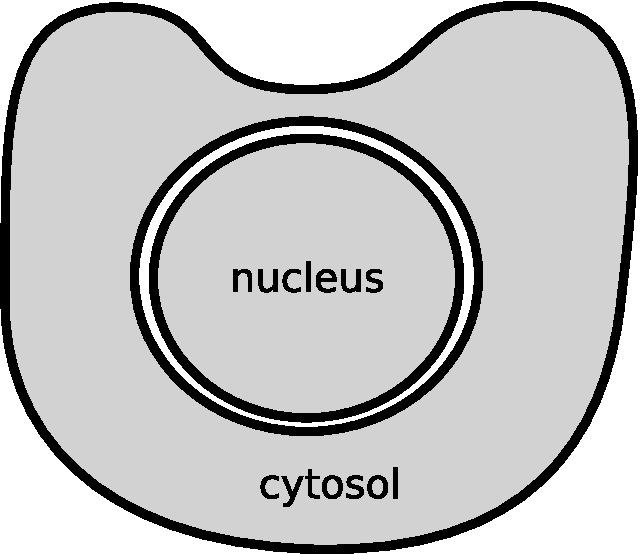
\includegraphics[scale = 0.4]{examples/compartment-cell}
 \includegraphics[scale = 0.4]{examples/compartment-cell-wrong}
  \caption{Compartments can surround other compartments; in that case, both of the compartment's borders must still be shown, with the result that the separation is drawn as two lines. The left example is correct, with twoo disjoint compartments representing the ``cytoplasm'' and the ``nucleus''. The right example is incorrect. Indeed the compartments ``cell'' and ``nucleus'' would be disjoint, the latter only overlapping the former. As a result, the volume of the nucleus is duplicated.}
  \label{fig:two-comp}
\end{figure}

The example diagram in \fig{three-comp} represents three adjacent compartments.  Two of the compartments carry units of information.  Notice that these units of information do not overlap multiple membrane boundaries.

\begin{figure}[H]
  \centering
  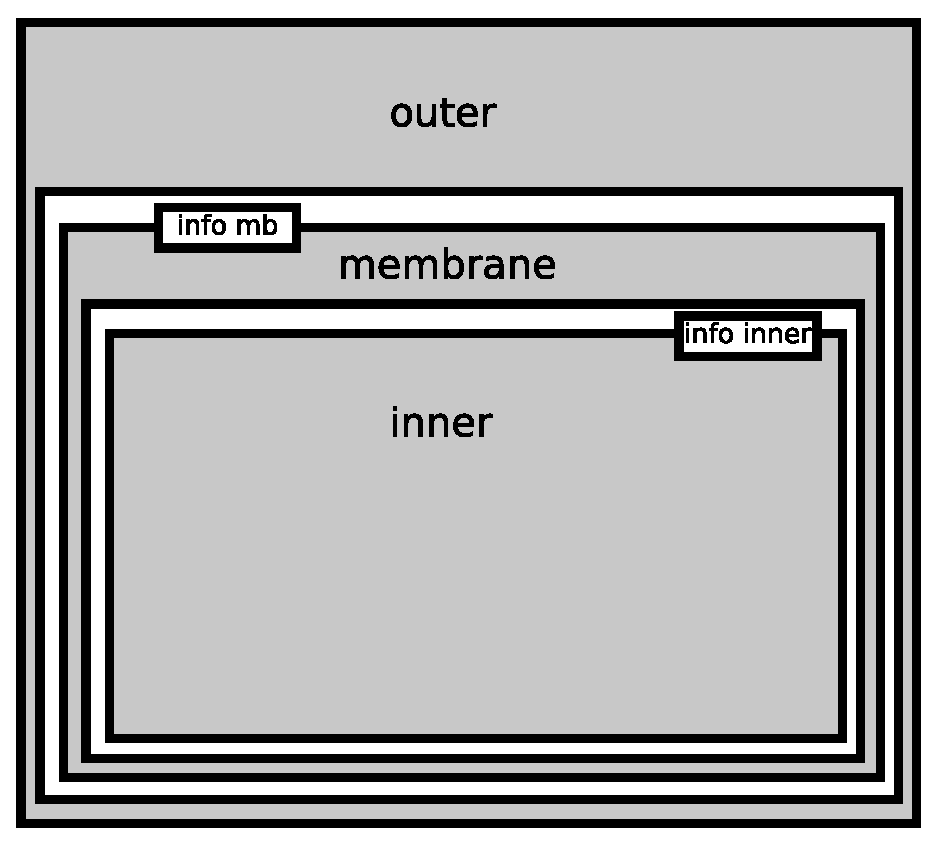
\includegraphics[scale = 0.4]{examples/compartment-3comp}
  \caption{Illustration of units of information and surrounding compartments.}
  \label{fig:three-comp}
\end{figure}

To allow more aesthetically pleasing and understandable diagrams, compartments are allowed to overlap each other visually, but it must be kept in mind that this does not mean the top compartment contains part of the bottom compartment.  \fig{overlap} shows two semantically equivalent placement of compartments:

\begin{figure}[H]
  \centering
  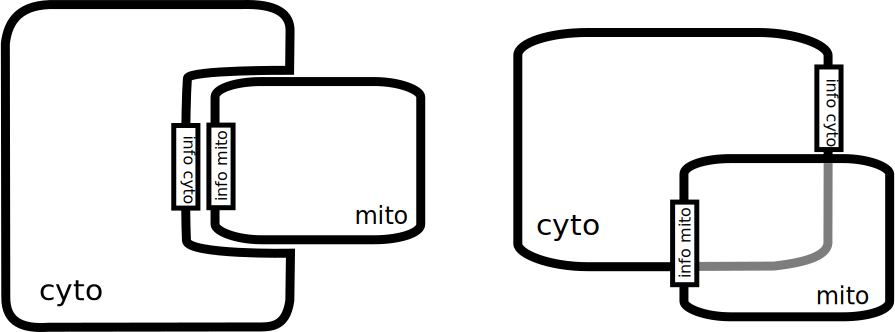
\includegraphics[scale = 0.4]{examples/compartment_overlapping}
  \caption{Overlapped compartments are permitted, but the overlap does not imply containment.}
  \label{fig:overlap}
\end{figure}

Overlapped (hidden) part of the compartment should not contain any object which could be covered by an overlapping compartment.  \fig{overlap-bad} illustrates the problem using an incorrect diagram.

\begin{figure}[H]
  \centering
  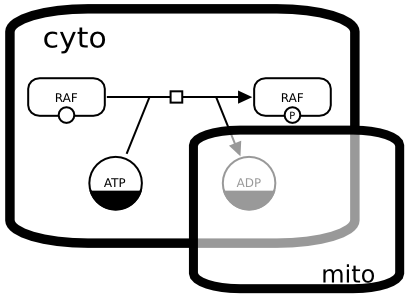
\includegraphics[scale = 0.45]{examples/compartment_overlapping_wrong}
  \caption{Example of an \textbf{incorrect} diagram.  Overlapped compartments must not obscure other objects.}
  \label{fig:overlap-bad}
\end{figure}





% The following is for [X]Emacs users.  Please leave in place.
% Local Variables:
% TeX-master: "../sbgn_PD-level1"
% End:
